\documentclass[11pt]{article}
\usepackage{setspace}
\usepackage{fullpage}
\usepackage{pslatex}
\usepackage{pgfplots}
\pgfplotsset{
	compat=1.4}
\usepackage{tikz}
\usetikzlibrary{shapes,arrows}
\let\word=\textit
\begin{document}
\begin{figure}[htb]
\centering
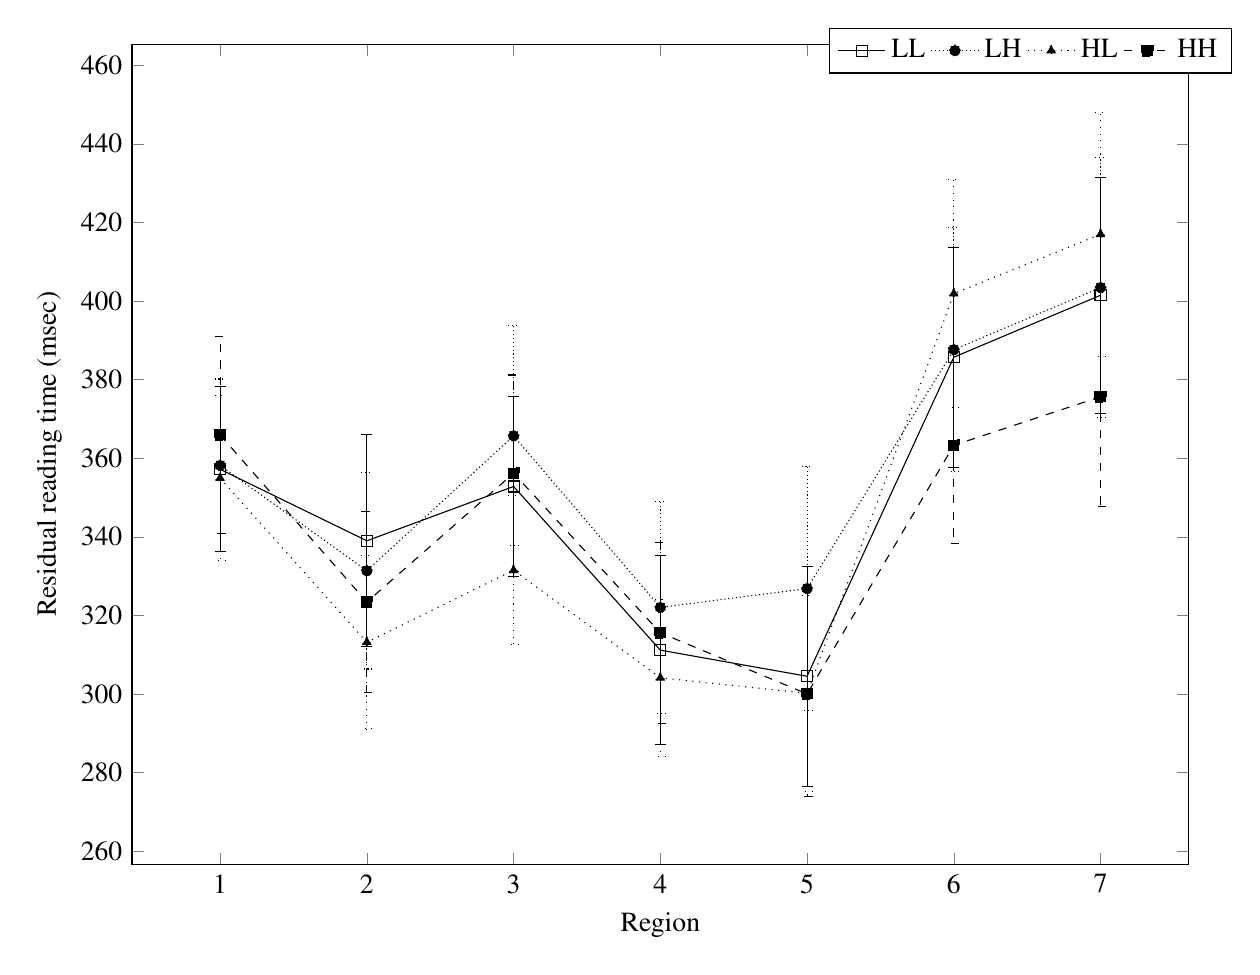
\begin{tikzpicture}
\begin{axis}[
	width=15cm, height=12cm,
	legend style={at={(0.85,1.02)},
	anchor=north,legend columns=-1},
	ylabel={Residual reading time (msec)},
	xlabel={Region},
	symbolic x coords={1, 2, 3, 4, 5, 6, 7},
    	xtick=data,
]
\addplot[
		mark=square,
		error bars/.cd,
		error bar style={color=black},
		y dir=both,
		y explicit
] 
	coordinates {(1, 357.182 ) +- ( 21 , 21 )(2, 338.991 ) +- ( 27 , 27 )(3, 352.8118 ) +- ( 23 , 23 )(4, 311.1529 ) +- ( 24 , 24 )(5, 304.5103 ) +- ( 28 , 28 )(6, 385.719 ) +- ( 28 , 28 )(7, 401.4799 ) +- ( 30 , 30 )};
\addplot[
		mark=*,
		densely dotted,
		error bars/.cd,
		error bar style={color=black},
		y dir=both,
		y explicit
] 
	coordinates {(1, 358.1686 ) +- ( 22 , 22 )(2, 331.3656 ) +- ( 25 , 25 )(3, 365.6897 ) +- ( 28 , 28 )(4, 322.0298 ) +- ( 27 , 27 )(5, 326.8356 ) +- ( 31 , 31 )(6, 387.6325 ) +- ( 31 , 31 )(7, 403.4297 ) +- ( 33 , 33 )};
\addplot[
		mark=triangle*,
		dotted,
		error bars/.cd,
		error bar style={color=black},
		y dir=both,
		y explicit
] 
	coordinates {(1, 354.9263 ) +- ( 21 , 21 )(2, 313.1588 ) +- ( 22 , 22 )(3, 331.4965 ) +- ( 19 , 19 )(4, 304.1205 ) +- ( 20 , 20 )(5, 300.1805 ) +- ( 25 , 25 )(6, 401.8872 ) +- ( 29 , 29 )(7, 417.0058 ) +- ( 31 , 31 )};
\addplot[
		mark=square*,
		dashed,
		error bars/.cd,
		error bar style={color=black},
		y dir=both,
		y explicit
] 
	coordinates {(1, 365.9319 ) +- ( 25 , 25 )(2, 323.4077 ) +- ( 23 , 23 )(3, 356.1855 ) +- ( 25 , 25 )(4, 315.5753 ) +- ( 23 , 23 )(5, 300.022 ) +- ( 26 , 26 )(6, 363.2937 ) +- ( 25 , 25 )(7, 375.644 ) +- ( 28 , 28 )};
\legend{LL,LH,HL,HH}
\end{axis}
\end{tikzpicture}
\caption{Mean residual reading times for all sentence regions}
\end{figure}
\end{document}